\chapter{Los números reales}
\label{ap:numeros-reales}
\index{Números reales}\index{Cortadura de Dedekind}\index{Sucesión de Cauchy}\index{Supremo}\index{Ínfimo}\index{Valor absoluto}\index{Propiedad arquimediana}\index{Densidad de los racionales}

\section{Construcción de los sistemas numéricos}

Antes de estudiar las propiedades de $\mathbb{R}$, conviene comprender cómo se construyen sistemáticamente los números a partir de los naturales. Cada extensión resuelve una ecuación que el sistema anterior no podía manejar.

\begin{center}
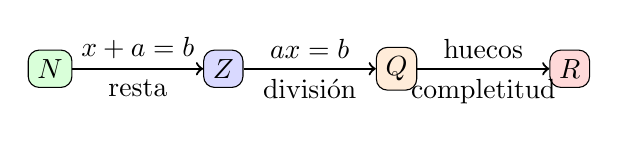
\begin{tikzpicture}[node distance=2.2cm, auto]
  \node[draw,rounded corners,fill=green!15] (N) {$\mathbb{N}$};
  \node[draw,rounded corners,fill=blue!15,right of=N] (Z) {$\mathbb{Z}$};
  \node[draw,rounded corners,fill=orange!15,right of=Z] (Q) {$\mathbb{Q}$};
  \node[draw,rounded corners,fill=red!15,right of=Q] (R) {$\mathbb{R}$};
  \draw[->,thick] (N) -- (Z) node[midway,above] {$x+a=b$} node[midway,below] {resta};
  \draw[->,thick] (Z) -- (Q) node[midway,above] {$ax=b$} node[midway,below] {división};
  \draw[->,thick] (Q) -- (R) node[midway,above] {huecos} node[midway,below] {completitud};
\end{tikzpicture}
\end{center}

\subsection{De \texorpdfstring{$\mathbb{N}$}{N} a \texorpdfstring{$\mathbb{Z}$}{Z}}

Los números naturales $\mathbb{N}$ se axiomatizan mediante los axiomas de Peano. En $\mathbb{N}$, la ecuación $x+a=b$ solo tiene solución cuando $a\leq b$. Para resolverla en general, se define $\mathbb{Z}$ como el conjunto de pares $(a,b)\in\mathbb{N}\times\mathbb{N}$ bajo la relación de equivalencia
\[
  (a,b)\sim(c,d)\quad\Longleftrightarrow\quad a+d=b+c.
\]
Intuitivamente, el par $(a,b)$ representa la ``diferencia'' $a-b$. La clase de $(a,b)$ se identifica con $a-b$, y las operaciones se definen representante a representante:
\[
  [(a,b)]+[(c,d)]=[(a+c,b+d)],\qquad [(a,b)]\cdot[(c,d)]=[(ac+bd,ad+bc)].
\]

\subsection{De \texorpdfstring{$\mathbb{Z}$}{Z} a \texorpdfstring{$\mathbb{Q}$}{Q}}

En $\mathbb{Z}$, la ecuación $ax=b$ ($a\neq 0$) no siempre tiene solución. Se define $\mathbb{Q}$ como el conjunto de pares $(p,q)\in\mathbb{Z}\times\mathbb{Z}$ con $q\neq 0$, bajo la relación
\[
  (p,q)\sim(r,s)\quad\Longleftrightarrow\quad ps=qr.
\]
La clase de $(p,q)$ se denota $\frac{p}{q}$, y las operaciones de cuerpo se definen de manera natural.

\subsection{De \texorpdfstring{$\mathbb{Q}$}{Q} a \texorpdfstring{$\mathbb{R}$}{R}}

Los números reales constituyen el escenario fundamental del análisis matemático. A diferencia de los números racionales, que surgen naturalmente de las operaciones aritméticas, los reales son una construcción intelectual cuyo objetivo es ``llenar los huecos'' de la recta racional. Presentamos dos construcciones clásicas ---las de Dedekind y Cantor--- y desarrollamos las propiedades que hacen de $\mathbb{R}$ un cuerpo ordenado completo.

\subsubsection{Cortaduras de Dedekind}

\begin{definition}
\label{def:cortadura}
Una \emph{cortadura} de Dedekind es un par $(A,B)$ de subconjuntos no vacíos de $\mathbb{Q}$ tales que:
\begin{enumerate}
  \item[(i)] $A\cup B=\mathbb{Q}$ y $A\cap B=\emptyset$.
  \item[(ii)] Si $a\in A$ y $q\in\mathbb{Q}$ con $q<a$, entonces $q\in A$.
  \item[(iii)] $A$ no tiene máximo.
\end{enumerate}
\end{definition}

La condición (iii) es la que distingue una cortadura de una simple partición: el ``corte'' ocurre donde debería estar un número real que no es racional.

\begin{example}
La cortadura que define $\sqrt{2}$ está dada por $A=\{q\in\mathbb{Q}:\,q^2<2\text{ o }q<0\}$ y $B=\mathbb{Q}\setminus A$.
\end{example}

\begin{definition}
\label{def:reales-dedekind}
El conjunto $\mathbb{R}$ de los números reales es el conjunto de todas las cortaduras de Dedekind.
\end{definition}

\subsubsection{Sucesiones de Cauchy}

\begin{definition}
\label{def:cauchy-racionales}
Una sucesión $(q_n)$ de números racionales es de \emph{Cauchy} si para todo $\varepsilon\in\mathbb{Q}^+$ existe $N\in\mathbb{N}$ tal que $|q_m-q_n|<\varepsilon$ siempre que $m,n\geq N$.
\end{definition}

\begin{definition}
\label{def:reales-cantor}
Definimos $\mathbb{R}$ como el conjunto de clases de equivalencia de sucesiones de Cauchy de racionales, donde $(q_n)\sim (r_n)$ si $\lim_{n\to\infty}|q_n-r_n|=0$.
\end{definition}

Ambas construcciones producen cuerpos ordenados isomorfos. La elección entre una u otra es cuestión de gusto; en el análisis funcional, la perspectiva de Cauchy (completitud métrica) es la que generaliza más naturalmente.

\section{Propiedades algebraicas y de orden}

\begin{theorem}
\label{teo:cuerpo-ordenado}
$\mathbb{R}$ es un \emph{cuerpo ordenado}: satisface los axiomas de cuerpo (asociatividad, conmutatividad, distributividad, elementos neutros e inversos) y los de orden (compatibilidad de la suma y el producto con el orden).
\end{theorem}

\begin{proof}[Bosquejo]
Las operaciones se definen término a término en las sucesiones de Cauchy (o mediante las cortaduras), y se verifica que las clases de equivalencia heredan las propiedades de $\mathbb{Q}$.
\end{proof}

\section{Suprema, ínfimos y completitud}

\begin{definition}
\label{def:supremo}
Sea $A\subseteq\mathbb{R}$ no vacío. Un número $M\in\mathbb{R}$ es una \emph{cota superior} de $A$ si $a\leq M$ para todo $a\in A$. El \emph{supremo} de $A$, denotado $\sup A$, es la mínima cota superior de $A$, si existe. Análogamente se define el \emph{ínfimo} $\inf A$ como la máxima cota inferior.
\end{definition}

\begin{theorem}[Completitud de Dedekind]
\label{teo:completitud-dedekind}
Todo subconjunto no vacío de $\mathbb{R}$ acotado superiormente posee supremo.
\end{theorem}

\begin{proof}
Dado $A\subseteq\mathbb{R}$ acotado superiormente, consideremos el conjunto $S$ de todas las cotas superiores de $A$. El par $(\mathbb{R}\setminus S, S)$ constituye una cortadura de Dedekind; el número real que representa es, por construcción, $\sup A$.
\end{proof}

\begin{theorem}[Caracterización del supremo]
\label{teo:carac-sup}
Sea $A\subseteq\mathbb{R}$ no vacío y $s\in\mathbb{R}$. Entonces $s=\sup A$ si y solo si:
\begin{enumerate}
  \item[(i)] $s$ es cota superior de $A$;
  \item[(ii)] para todo $\varepsilon>0$, existe $a\in A$ tal que $s-\varepsilon<a\leq s$.
\end{enumerate}
\end{theorem}

\begin{proof}
Si $s=\sup A$, entonces (i) es inmediata. Si (ii) fallara para algún $\varepsilon>0$, entonces $s-\varepsilon$ sería cota superior, contradiciendo la minimalidad de $s$. Recíprocamente, si $s$ satisface (i) y (ii), cualquier cota superior $M<s$ no puede cumplir (ii) para $\varepsilon=s-M$.
\end{proof}

\section{Valor absoluto y desigualdades fundamentales}

\begin{definition}
\label{def:valor-absoluto}
El \emph{valor absoluto} de $x\in\mathbb{R}$ se define por
\[
  |x|=\begin{cases}x & \text{si }x\geq 0,\\ -x & \text{si }x<0.\end{cases}
\]
\end{definition}

\begin{proposition}
\label{prop:prop-abs}
Para todo $x,y\in\mathbb{R}$:
\begin{enumerate}
  \item[(i)] $|x|\geq 0$, y $|x|=0\Leftrightarrow x=0$.
  \item[(ii)] $|xy|=|x|\,|y|$.
  \item[(iii)] $|x+y|\leq |x|+|y|$ (desigualdad triangular).
  \item[(iv)] $||x|-|y||\leq |x-y|$.
\end{enumerate}
\end{proposition}

\begin{proof}
La propiedad (iii) es la más relevante. Si $x+y\geq 0$, entonces $|x+y|=x+y\leq|x|+|y|$. Si $x+y<0$, entonces $|x+y|=-(x+y)=(-x)+(-y)\leq|x|+|y|$.
\end{proof}

\section{Propiedad arquimediana}

\begin{theorem}[Propiedad arquimediana]
\label{teo:arquimediana}
Para cualesquiera $x,y\in\mathbb{R}$ con $x>0$, existe $n\in\mathbb{N}$ tal que $nx>y$.
\end{theorem}

\begin{proof}
Si no existiera tal $n$, entonces $y$ sería cota superior de $\{nx:\,n\in\mathbb{N}\}$. Sea $s=\sup\{nx:\,n\in\mathbb{N}\}$. Entonces $s-x<s$, luego existe $n$ tal que $nx>s-x$, es decir, $(n+1)x>s$, contradicción.
\end{proof}

\begin{center}
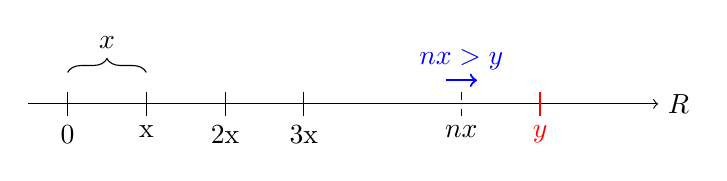
\begin{tikzpicture}[scale=1.0]
  \draw[->] (-0.5,0) -- (7.5,0) node[right] {$\mathbb{R}$};
  \foreach \x/\n in {0/0,1/x,2/2x,3/3x}
    \draw (\x,0.15) -- (\x,-0.15) node[below] {\n};
  \draw[dashed] (5,0.15) -- (5,-0.15) node[below] {$nx$};
  \draw[thick,red] (6,0.15) -- (6,-0.15) node[below] {$y$};
  \draw[decorate,decoration={brace,amplitude=5pt}] (0,0.4) -- (1,0.4) node[midway,above=5pt] {$x$};
  \draw[->,thick,blue] (4.8,0.3) -- (5.2,0.3) node[above,midway] {$nx>y$};
\end{tikzpicture}
\end{center}

\begin{corollary}
\label{cor:racionales-densos-orden}
Para todo $\varepsilon>0$ existe $n\in\mathbb{N}$ tal que $1/n<\varepsilon$.
\end{corollary}

\section{Densidad de \texorpdfstring{$\mathbb{Q}$}{Q} y de los irracionales}

\begin{theorem}[Densidad de los racionales]
\label{teo:densidad-q}
Entre dos números reales distintos existe al menos un número racional. Equivalentemente, para todo $x\in\mathbb{R}$ y todo $\varepsilon>0$ existe $q\in\mathbb{Q}$ tal que $|x-q|<\varepsilon$.
\end{theorem}

\begin{proof}
Sea $x<y$. Por la propiedad arquimediana, existe $n\in\mathbb{N}$ tal que $n(y-x)>1$. Sea $m$ el menor entero tal que $m>nx$. Entonces $nx<m\leq nx+1<ny$, luego $x<m/n<y$.
\end{proof}

\begin{center}
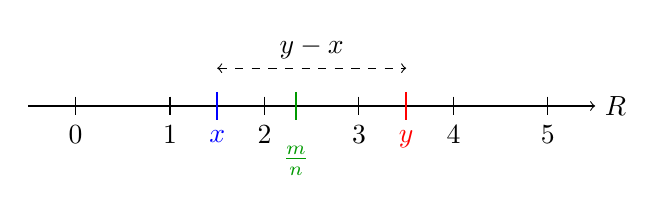
\begin{tikzpicture}[scale=1.2]
  \draw[->] (-0.5,0) -- (5.5,0) node[right] {$\mathbb{R}$};
  \foreach \x in {0,1,2,3,4,5}
    \draw (\x,0.1) -- (\x,-0.1) node[below] {\x};
  \draw[thick,blue] (1.5,0.15) -- (1.5,-0.15) node[below] {$x$};
  \draw[thick,red] (3.5,0.15) -- (3.5,-0.15) node[below] {$y$};
  \draw[thick,green!60!black] (2.333,0.15) -- (2.333,-0.15) node[below=0.2cm] {$\frac{m}{n}$};
  \draw[<->,dashed] (1.5,0.4) -- (3.5,0.4) node[midway,above] {$y-x$};
\end{tikzpicture}
\end{center}

\begin{corollary}[Densidad de los irracionales]
\label{cor:densidad-irracionales}
Entre dos números reales distintos existe al menos un número irracional.
\end{corollary}
\begin{proof}
Si $x<y$, entonces $x-\sqrt{2}<y-\sqrt{2}$. Por densidad de $\mathbb{Q}$, existe $q\in\mathbb{Q}\cap(x-\sqrt{2},y-\sqrt{2})$. Luego $q+\sqrt{2}$ es irracional y pertenece a $(x,y)$.
\end{proof}

\begin{remark}
La densidad implica que cualquier número real puede aproximarse arbitrariamente por racionales e irracionales. Esta propiedad es esencial para definir funciones mediante prolongación por continuidad y para la teoría de la integración.
\end{remark}

\section{Intervalos encajados y completitud}

La completitud de $\mathbb{R}$ puede formularse de múltiples maneras equivalentes. Una de las más intuitivas es el principio de los intervalos encajados.

\begin{theorem}[Principio de los intervalos encajados de Cantor]
\label{teo:intervalos-encajados}
Sea $(I_n)$ una sucesión de intervalos cerrados y acotados $I_n=[a_n,b_n]$ tales que $I_{n+1}\subseteq I_n$ para todo $n$. Entonces $\bigcap_{n=1}^{\infty} I_n\neq\emptyset$.
\end{theorem}

\begin{proof}
La sucesión $(a_n)$ es creciente y acotada superiormente por $b_1$. Por completitud de Dedekind, existe $a=\sup a_n$. Análogamente, $(b_n)$ es decreciente y acotada inferiormente, luego existe $b=\inf b_n$. Como $a_n\leq b_n$ para todo $n$, se tiene $a\leq b$, y por tanto $[a,b]\subseteq\bigcap I_n$.
\end{proof}

\begin{center}
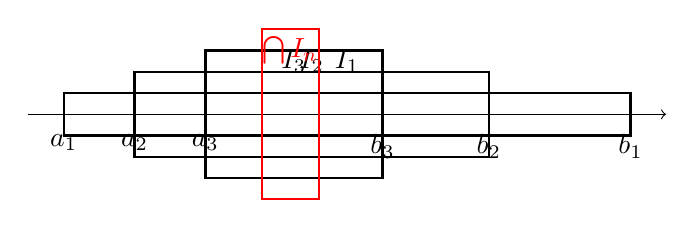
\begin{tikzpicture}[scale=0.9]
  \draw[->] (-0.5,0) -- (8.5,0);
  \draw[thick] (0,0.3) rectangle (8,-0.3) node[midway,above=0.4cm] {$I_1$};
  \draw[thick] (1,0.6) rectangle (6,-0.6) node[midway,above=0.4cm] {$I_2$};
  \draw[thick] (2,0.9) rectangle (4.5,-0.9) node[midway,above=0.4cm] {$I_3$};
  \draw[thick,red] (2.8,1.2) rectangle (3.6,-1.2) node[midway,above=0.5cm] {$\bigcap I_n$};
  \foreach \x/\n in {0/a_1,8/b_1,1/a_2,6/b_2,2/a_3,4.5/b_3}
    \draw (\x,0.15) -- (\x,-0.15) node[below] {$\n$};
\end{tikzpicture}
\end{center}

\begin{remark}
Si además la longitud $b_n-a_n\to 0$, entonces $\bigcap I_n$ consiste en un único punto. Esta versión fuerte se utiliza para demostrar la no numerabilidad de $\mathbb{R}$ y para construir funciones continuas nowhere-differentiable.
\end{remark}

\section{Completitud de Cauchy}

La completitud de $\mathbb{R}$ es la propiedad que distingue al análisis real del análisis sobre los racionales. Garantiza que los ``huecos'' de $\mathbb{Q}$ han sido colmatados.

\begin{theorem}[Completitud de $\mathbb{R}$]
\label{teo:completitud-r}
Toda sucesión de Cauchy en $\mathbb{R}$ converge a un límite en $\mathbb{R}$.
\end{theorem}

\begin{proof}[Bosquejo]
Sea $(x_n)$ de Cauchy. La sucesión está acotada, luego posee una subsucesión convergente (Bolzano--Weierstrass, que se prueba a partir de la completitud de Dedekind). Una sucesión de Cauchy con una subsucesión convergente es ella misma convergente.
\end{proof}

\begin{remark}
La completitud de $\mathbb{R}$ puede formularse de múltiples maneras equivalentes: completitud de Dedekind, completitud de Cauchy, principio de los intervalos encajados de Cantor, teorema de Bolzano--Weierstrass, y teorema de Heine--Borel para intervalos cerrados. Esta redundancia de formulaciones equivalentes es característica de las propiedades estructurales profundas.
\end{remark}

\section{La recta real extendida}

Es útil adjuntar a $\mathbb{R}$ dos símbolos $+\infty$ y $-\infty$ que representan los extremos ideales de la recta.

\begin{definition}
La \emph{recta real extendida} es $\overline{\mathbb{R}}=\mathbb{R}\cup\{-\infty,+\infty\}$. Se extiende el orden declarando $-\infty<x<+\infty$ para todo $x\in\mathbb{R}$. Las operaciones aritméticas con $\pm\infty$ se definen con las convenciones naturales, salvo las formas indeterminadas $\infty-\infty$, $0\cdot\infty$, $\infty/\infty$ y $0/0$.
\end{definition}

\begin{example}
En $\overline{\mathbb{R}}$, todo subconjunto tiene supremo e ínfimo. En particular, $\sup\emptyset=-\infty$ y $\inf\emptyset=+\infty$.
\end{example}

\section{Sucesiones reales elementales}

Aunque el estudio sistemático de las sucesiones corresponde al \cref{ch:sucesiones}, introducimos aquí algunos ejemplos paradigmáticos que ilustran las propiedades de $\mathbb{R}$.

\begin{example}[Serie armónica]
La serie $\sum_{n=1}^{\infty}\frac{1}{n}$ diverge. En efecto, agrupando términos
\[
  1+\frac{1}{2}+\Bigl(\frac{1}{3}+\frac{1}{4}\Bigr)+\Bigl(\frac{1}{5}+\cdots+\frac{1}{8}\Bigr)+\cdots
  \geq 1+\frac{1}{2}+\frac{1}{2}+\frac{1}{2}+\cdots
\]
se obtienen sumas parciales arbitrariamente grandes. Este hecho muestra que en $\mathbb{R}$, una sucesión creciente no siempre converge: necesita estar acotada.
\end{example}

\begin{example}[Serie armónica alternada]
La serie $\sum_{n=1}^{\infty}\frac{(-1)^{n+1}}{n}=1-\frac{1}{2}+\frac{1}{3}-\frac{1}{4}+\cdots$ converge a $\log 2$. Esta convergencia condicional (no absoluta) será demostrada en el \cref{ch:series} mediante el criterio de Leibniz.
\end{example}

\begin{example}[Sucesión de Fibonacci y razón áurea]
Definida por $F_1=F_2=1$ y $F_{n+2}=F_{n+1}+F_n$, la sucesión de Fibonacci satisface
\[
  \lim_{n\to\infty}\frac{F_{n+1}}{F_n}=\varphi=\frac{1+\sqrt{5}}{2}\approx 1.618\dots
\]
El número $\varphi$, llamado \emph{razón áurea}, es irracional. Este límite puede probarse resolviendo la ecuación característica $r^2=r+1$.
\end{example}

\section{Ejercicios}

\begin{exercise}
Demuestre que si $A\subseteq\mathbb{R}$ es no vacío y acotado inferiormente, entonces $\inf A$ existe.
\end{exercise}

\begin{exercise}
Pruebe que todo número real es límite de una sucesión de números racionales.
\end{exercise}

\begin{exercise}
Sea $A\subseteq\mathbb{R}$ no vacío, acotado superiormente, y tal que $\sup A\notin A$. Demuestre que existe una sucesión estrictamente creciente en $A$ que converge a $\sup A$.
\end{exercise}

\begin{exercise}
Use el principio de los intervalos encajados para probar que $[0,1]$ no es numerable.
\end{exercise}

\begin{exercise}
Demuestre que la sucesión $x_n=(1+\frac{1}{n})^n$ es creciente y acotada superiormente (por ejemplo, por 3), luego converge. El límite es el número $e$. (Sugerencia: use el binomio de Newton y compare término a término con $x_{n+1}$.)
\end{exercise}

\begin{exercise}
Sea $a_1=1$ y $a_{n+1}=\sqrt{2+a_n}$. Demuestre que $(a_n)$ converge y calcule su límite. Sugerencia: pruebe por inducción que $a_n\leq 2$ y que $(a_n)$ es creciente.
\end{exercise}

\begin{exercise}
Demuestre que entre dos números reales distintos hay infinitos racionales e infinitos irracionales.
\end{exercise}

\begin{exercise}
Sea $x\in\mathbb{R}$. Demuestre que existe una única sucesión $(d_n)$ con $d_n\in\{0,1,\dots,9\}$ tal que $x=\sum_{n=1}^{\infty}d_n10^{-n}$ y que la sucesión no termina en una cola de nueves. Esto justifica rigurosamente la expansión decimal.
\end{exercise}

\begin{exercise}
Demuestre que $\sqrt{2}+\sqrt{3}$ es irracional. Sugerencia: si fuera racional, entonces $(\sqrt{2}+\sqrt{3})^2$ también lo sería, lo que lleva a una contradicción.
\end{exercise}

\begin{exercise}
Sea $(x_n)$ una sucesión de Cauchy. Demuestre que $(x_n)$ está acotada. Use esto para dar una demostración directa (sin Bolzano--Weierstrass) de que toda sucesión de Cauchy en $\mathbb{R}$ converge. (Sugerencia: tome una subsucesión que converja a $\limsup x_n$.)
\end{exercise}

\begin{problem}
Un conjunto $A\subseteq\mathbb{R}$ se dice \emph{inductivo} si $1\in A$ y $x\in A\Rightarrow x+1\in A$. Sea $\mathbb{N}'=\bigcap\{A\subseteq\mathbb{R}:\,A\text{ inductivo}\}$. Demuestre que $\mathbb{N}'$ satisface el principio de inducción matemática y que coincide con el conjunto de los números naturales usuales.
\end{problem}

\begin{problem}
Demuestre que el conjunto de los números de Liouville (reales que pueden aproximarse ``demasiado bien'' por racionales) es denso en $\mathbb{R}$ pero de medida nula. Este resultado conecta la teoría de números con la teoría de la medida.
\end{problem}
